\chapter{PANDUAN PENGGUNAAN}\label{bab:panduan}

\section{Kebutuhan Sistem}
Studio web cukup dijalankan di laptop Windows biasa; GPU hanya dibutuhkan untuk melatih ulang model dengan data penuh (Tabel~\ref{tab:kebutuhan}). FFmpeg tidak perlu dipasang terpisah karena paket \kode{imageio-ffmpeg} membawa program ffmpeg sendiri.

\begin{table}[htbp]
\centering
\singlespacing\small
\caption{Kebutuhan sistem.}
\label{tab:kebutuhan}
\begin{tabularx}{\textwidth}{L{2.6cm} L{4.6cm} Y}
\toprule
Komponen & Kebutuhan & Catatan\\
\midrule
Sistem operasi & Windows 10/11 64-bit & Kode juga berjalan di Linux (dipakai di Google Colab)\\
Python & 3.11 atau lebih baru, 64-bit & Diuji dengan Python 3.14\\
RAM & 8 GB & 16 GB disarankan untuk pelatihan lokal\\
Disk & $\pm$1 GB untuk kode dan environment & Dataset dan cache fitur membutuhkan puluhan GB\\
GPU & Opsional & Pelatihan penuh dijalankan di Google Colab\\
Paket Python & torch, numpy, librosa, soundfile, scikit-learn, pytest, imageio-ffmpeg & Tercantum di \kode{requirements.txt}\\
\bottomrule
\end{tabularx}
\end{table}

\section{Instalasi}\label{sec:instalasi}
Jalankan perintah berikut di PowerShell dari folder proyek hasil \kode{git clone}:
\begin{enumerate}
\item Buat environment Python dan perbarui pip:
\begin{Perintah}
py -3.14 -m venv .venv
.\.venv\Scripts\python.exe -m pip install --upgrade pip
\end{Perintah}
\item Pasang PyTorch sesuai petunjuk di \url{https://pytorch.org/get-started/locally/}; versi CPU cukup untuk studio web.
\item Pasang paket lainnya:
\begin{Perintah}
.\.venv\Scripts\python.exe -m pip install -r requirements.txt
\end{Perintah}
\item Jalankan tes otomatis. Hasil yang diharapkan: 42 tes lulus.
\begin{Perintah}
.\.venv\Scripts\python.exe -m pytest -q
\end{Perintah}
\end{enumerate}
Simpan daftar versi paket dengan \kode{pip freeze > environment-lock.txt} setiap kali menjalankan eksperimen agar hasilnya dapat diulang.

Model final sudah disertakan di repositori pada folder \kode{runs/hmf-aug-v2/}, sehingga studio dapat langsung dipakai setelah instalasi tanpa melatih ulang. Hanya file yang diperlukan yang disimpan (Tabel~\ref{tab:file-model}); file indeks cache berukuran $\pm$282 MB dan \kode{last.pt} tidak disertakan karena hanya dipakai saat pelatihan dan bisa dibuat ulang.

\begin{table}[htbp]
\centering
\singlespacing\small
\caption{File model final di repositori.}
\label{tab:file-model}
\begin{tabularx}{\textwidth}{L{5.1cm} L{1.4cm} Y}
\toprule
File & Ukuran & Kegunaan\\
\midrule
\kode{best.pt} & 0,1 MB & Bobot CNN terbaik (epoch 27); wajib untuk analisis\\
\kode{report.json} & 0,9 MB & Konfigurasi audio, arsitektur, dan metrik test; wajib untuk analisis dan panel model\\
\kode{history.json} & 0,04 MB & Loss dan metrik per epoch\\
\kode{cache\_audio\_config.json},\newline \kode{cache\_prepare\_config.json} & $<$0,01 MB & Pengaturan ekstraksi fitur saat pelatihan\\
\kode{cache\_skipped.json} & $<$0,01 MB & Daftar lagu yang gagal didekode saat pra-pemrosesan\\
\kode{manifest-musebench.csv} & 1,1 MB & Daftar lagu MUSEBENCH yang dipakai\\
\bottomrule
\end{tabularx}
\end{table}

\section{Menjalankan Studio Web}
Studio web dibuka dengan satu perintah, lalu dipakai lewat browser di alamat \url{http://127.0.0.1:8765}. Server hanya menerima koneksi dari komputer yang sama.
\begin{enumerate}
\item Buka PowerShell di folder proyek, lalu jalankan studio. Tanpa opsi, server memakai model terbaru di folder \kode{runs/}; opsi \kode{--run} memilih model tertentu.
\begin{Perintah}
.\.venv\Scripts\python.exe -m hmf.web --run runs/hmf-aug-v2
\end{Perintah}
\item Terminal menampilkan nama model aktif dan alamat studio. Buka alamat itu di browser (Gambar~\ref{fig:halaman-awal}).
\item Tarik file audio ke kotak unggah atau klik kotak itu untuk memilih file. Nama file dan pemutar audio akan tampil (Gambar~\ref{fig:file-dipilih}).
\item Klik \textbf{Analisis rekaman}. Lagu 3 menit biasanya selesai dalam beberapa detik di CPU.
\item Hentikan server dengan Ctrl+C di terminal.
\end{enumerate}
Pojok kanan atas halaman selalu menampilkan nama model yang aktif. Jika port 8765 sudah dipakai, misalnya karena studio lain masih berjalan, server menolak berjalan dan menyarankan memakai \kode{--port} lain.

\begin{figure}[htbp]
\centering
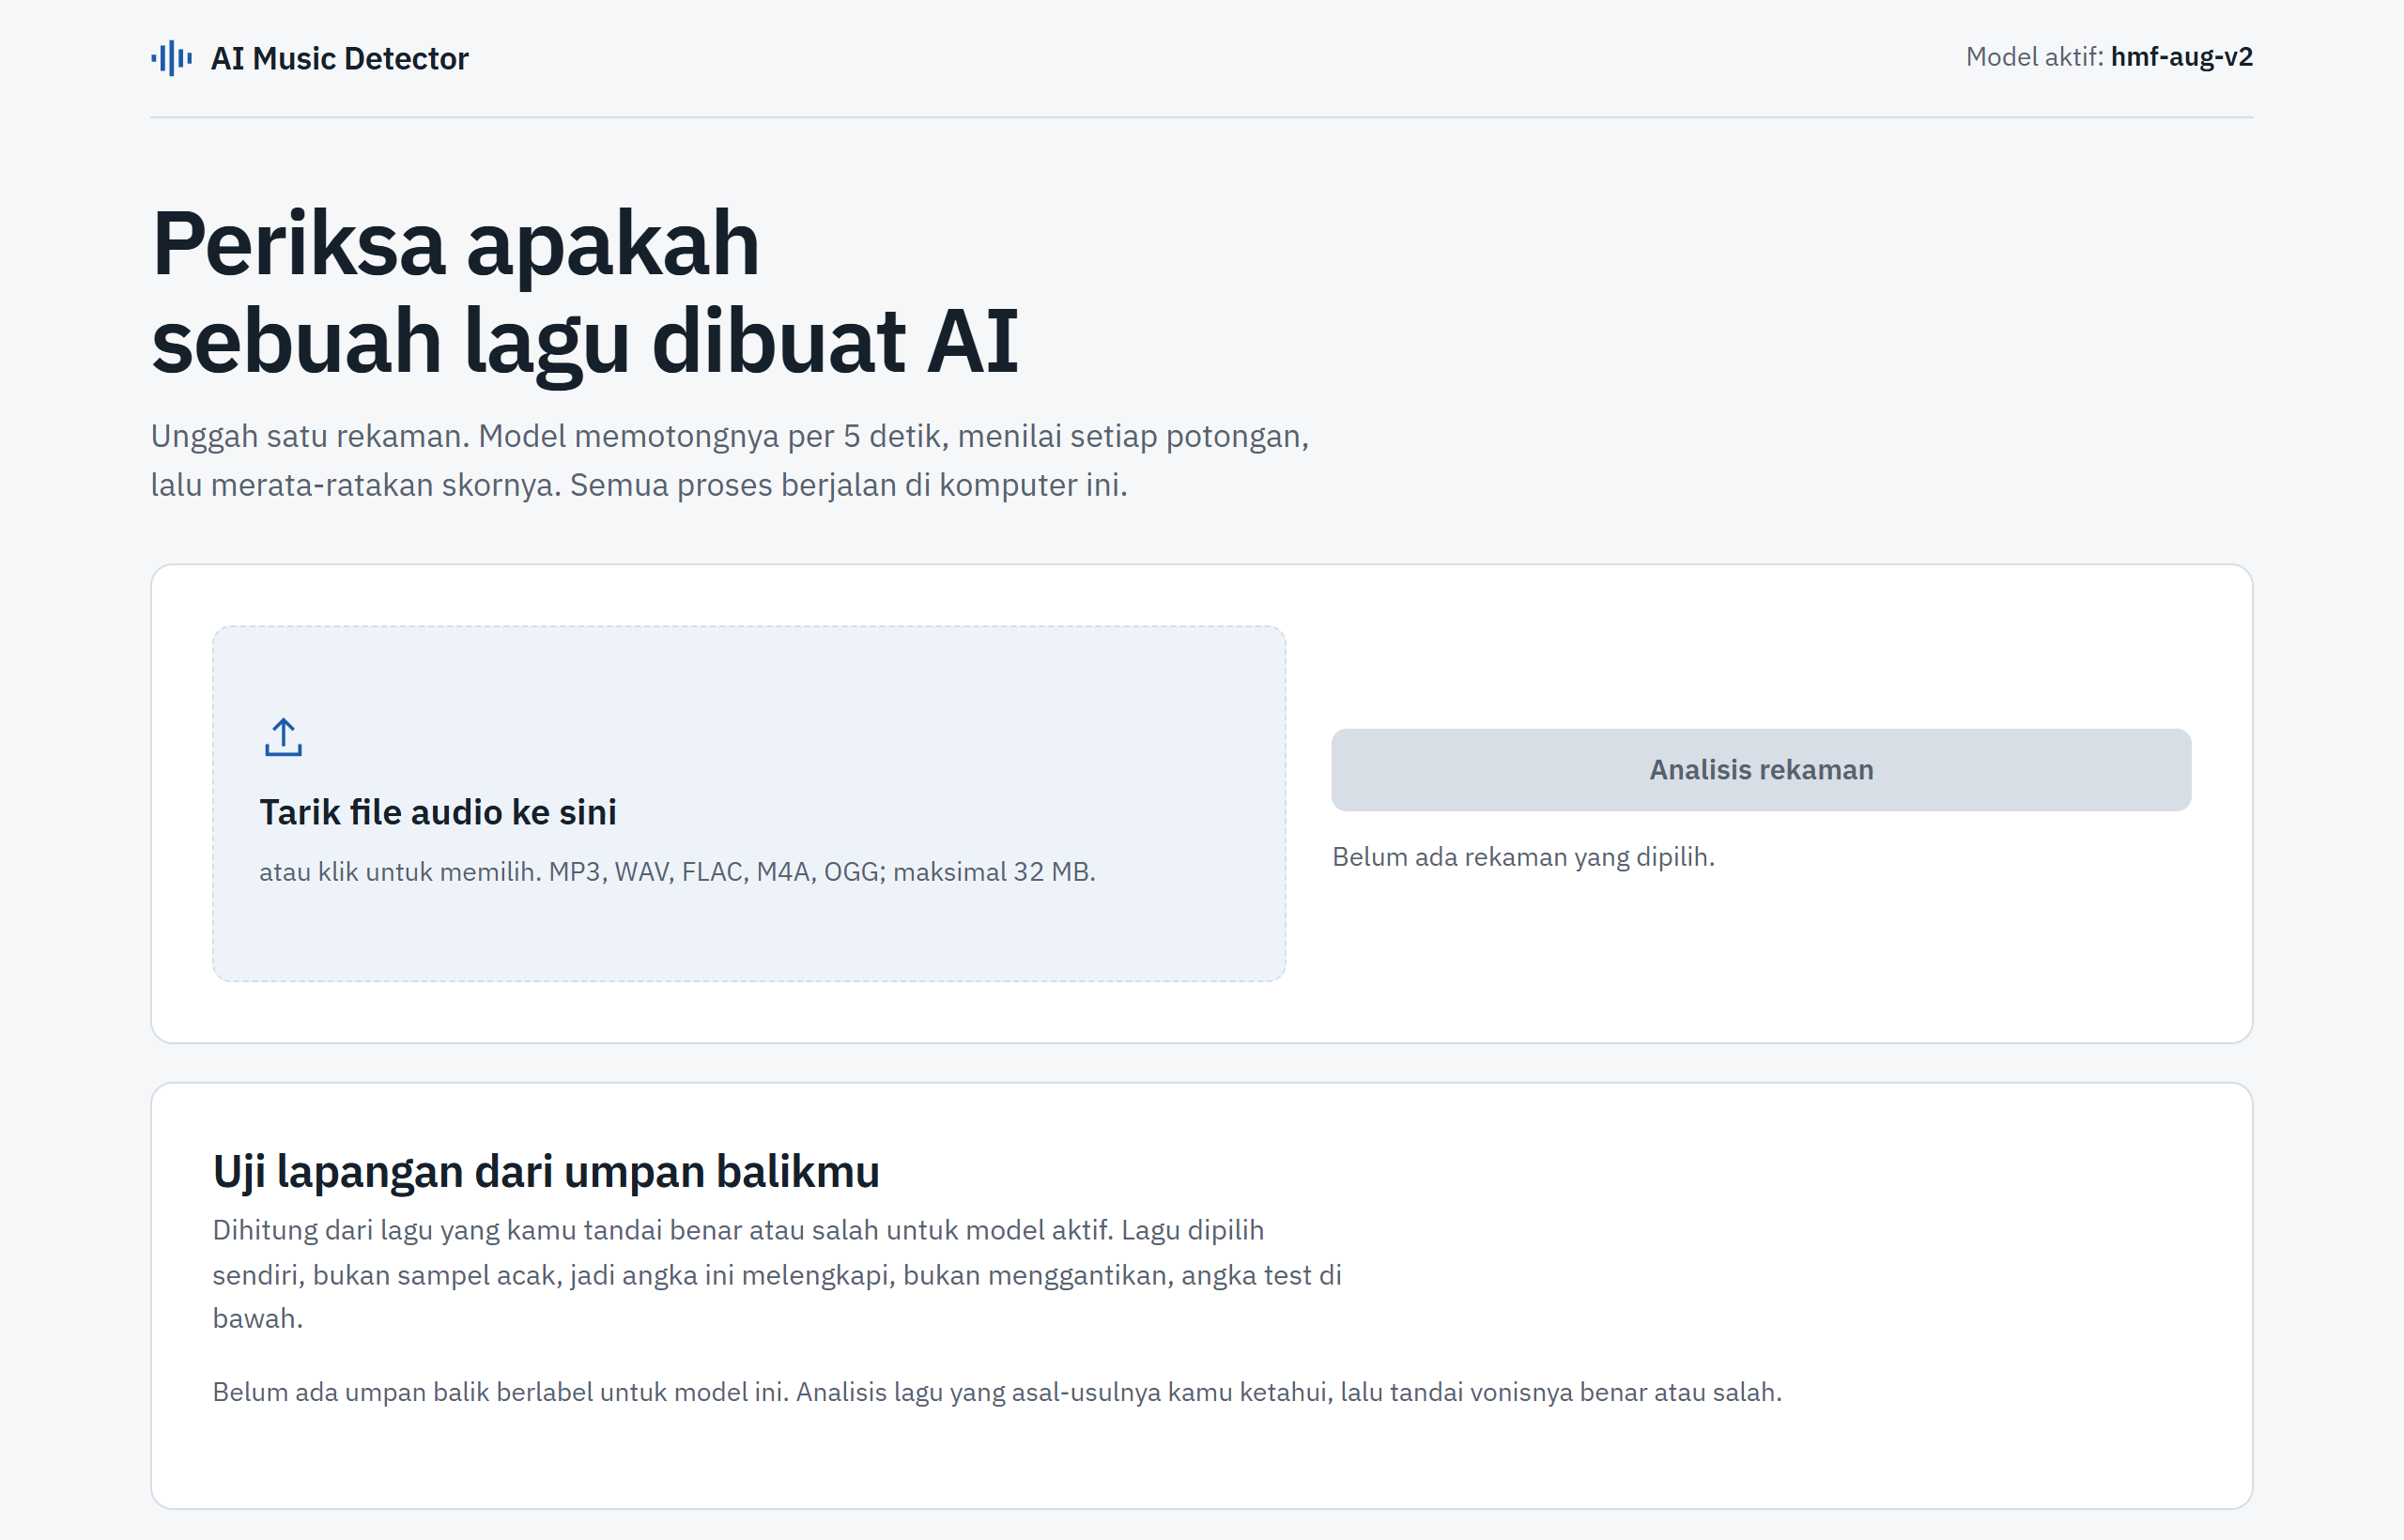
\includegraphics[width=0.95\textwidth]{01-halaman-awal.png}
\caption{Halaman awal studio dengan kotak unggah dan nama model aktif.}
\label{fig:halaman-awal}
\end{figure}

\begin{figure}[htbp]
\centering
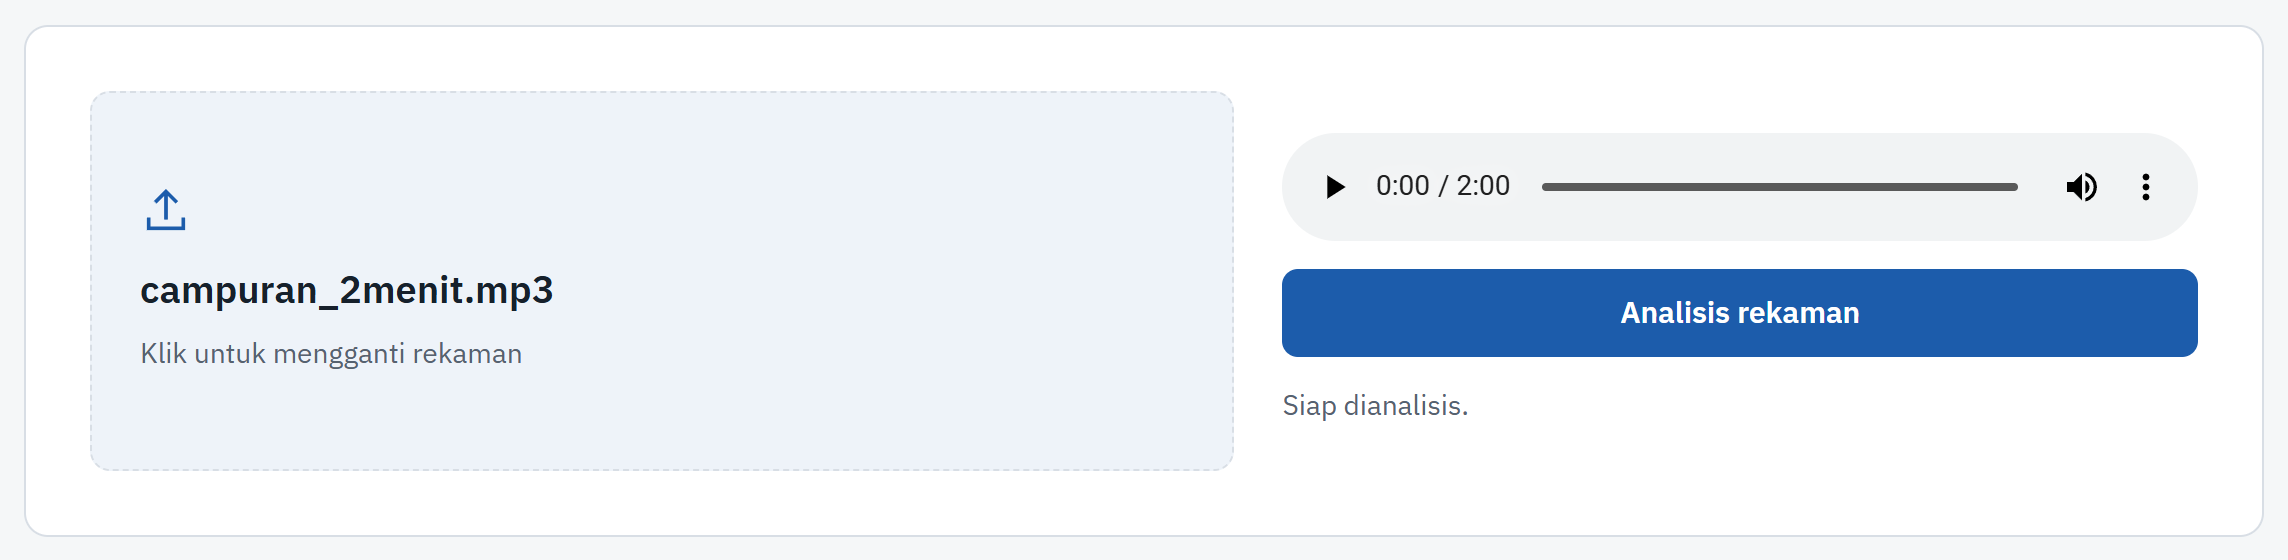
\includegraphics[width=0.95\textwidth]{02-file-dipilih.png}
\caption{Kotak unggah setelah file dipilih.}
\label{fig:file-dipilih}
\end{figure}

\section{Membaca Hasil Analisis}
Vonis ditentukan oleh satu angka: rata-rata skor AI semua segmen 5 detik. Jika rata-rata itu mencapai ambang 50\%, vonisnya AI; jika di bawahnya, Human. Tabel~\ref{tab:bagian-layar} menjelaskan setiap bagian layar hasil. Gambar pada subbab ini menunjukkan tata letak tampilan; angka di dalamnya berbeda untuk setiap lagu.

{\singlespacing\small
\begin{longtable}{L{2.6cm} L{4.6cm} L{5.1cm}}
\caption{Bagian layar hasil analisis.}\label{tab:bagian-layar}\\
\toprule
Bagian layar & Isi & Cara membacanya\\
\midrule
\endfirsthead
\toprule
Bagian layar & Isi & Cara membacanya\\
\midrule
\endhead
\bottomrule
\endfoot
Vonis & Kata \textbf{AI} (oranye) atau \textbf{Human} (biru) & Hasil akhir model untuk seluruh rekaman\\
Skor AI & Persentase, misalnya 51,46\% & Rata-rata skor segmen; makin dekat 100\% makin mirip data AI\\
\kode{ai\_score} & Angka mentah, misalnya 0.5146298917631308 & Nilai yang sama persis dengan di JSON\\
Meter & Batang 0--100\% dengan garis di ambang & Jarak ujung batang ke garis menunjukkan seberapa yakin vonisnya\\
Spektrogram & Energi per frekuensi (0--7 kHz) terhadap waktu & Persis masukan yang dilihat CNN\\
Skor per segmen & Satu batang per 5 detik, oranye jika $\ge$ ambang & Menunjukkan bagian lagu yang mendorong vonis\\
Pilih segmen & Penggeser dan teks keterangan & Pemutar audio melompat ke awal segmen yang dipilih\\
Data JSON & Laporan lengkap & Dapat dilihat atau diunduh untuk dokumentasi\\
\end{longtable}}

Persentase dibulatkan dua desimal tanpa melewati ambang atau batas: skor 0,49996 tampil 49,99\% (bukan 50,00\%), skor sangat kecil tampil $<$0,01\%, dan skor hampir 1 tampil $>$99,99\%. Spektrogram dan batang skor memakai sumbu waktu yang sama. Arahkan kursor ke batang untuk melihat nomor segmen, rentang waktu, dan skornya, lalu klik untuk memilih segmen.

Gambar~\ref{fig:vonis} dan~\ref{fig:spektrogram} memperlihatkan hasil untuk rekaman campuran 2 menit. Enam segmen pertama (lagu FMA) berada di bawah ambang, sedangkan sebagian besar segmen berikutnya (lagu Udio dan Suno) di atas ambang. Rata-ratanya 51,46\%, sehingga vonisnya AI dengan selisih tipis. Vonis setipis ini sebaiknya dibaca bersama grafik segmen, bukan sebagai kepastian.

\begin{figure}[htbp]
\centering
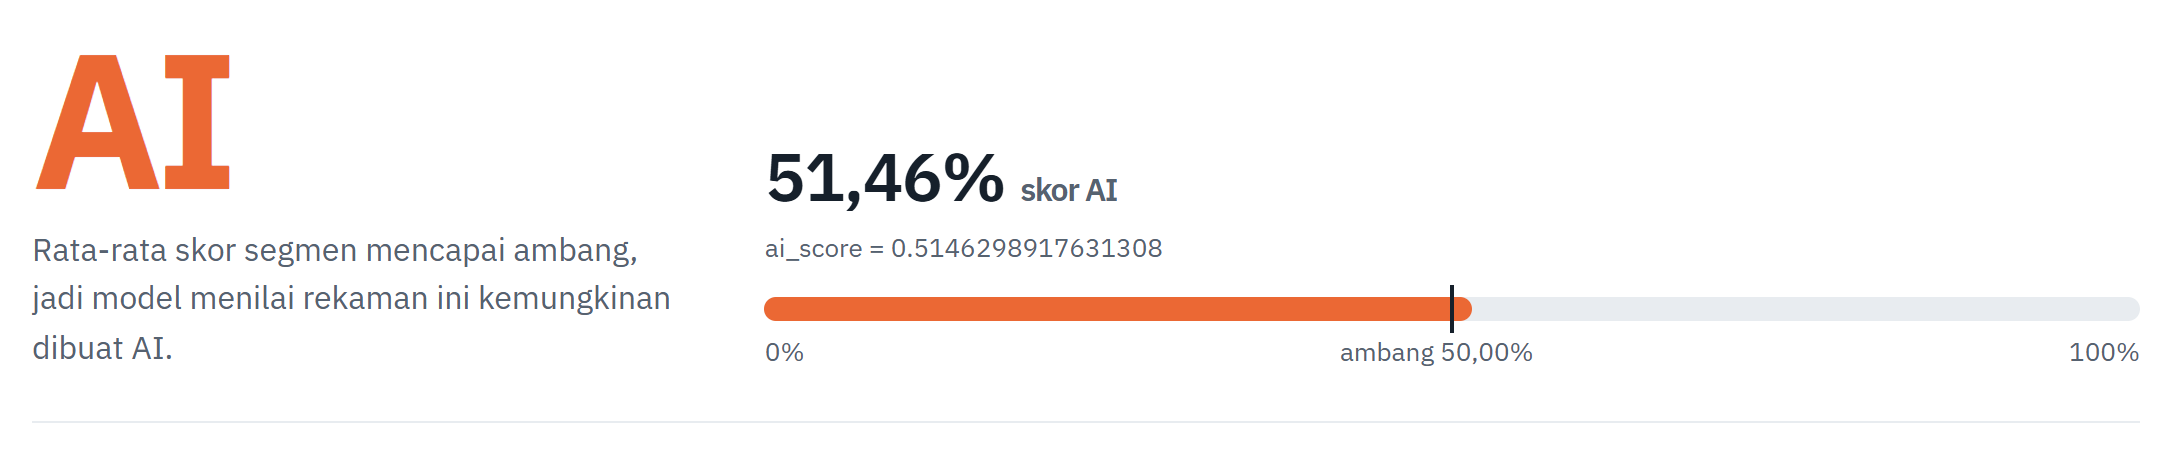
\includegraphics[width=0.95\textwidth]{03-hasil-vonis.png}
\caption{Vonis, skor AI, nilai \kode{ai\_score}, dan meter terhadap ambang.}
\label{fig:vonis}
\end{figure}

\begin{figure}[htbp]
\centering
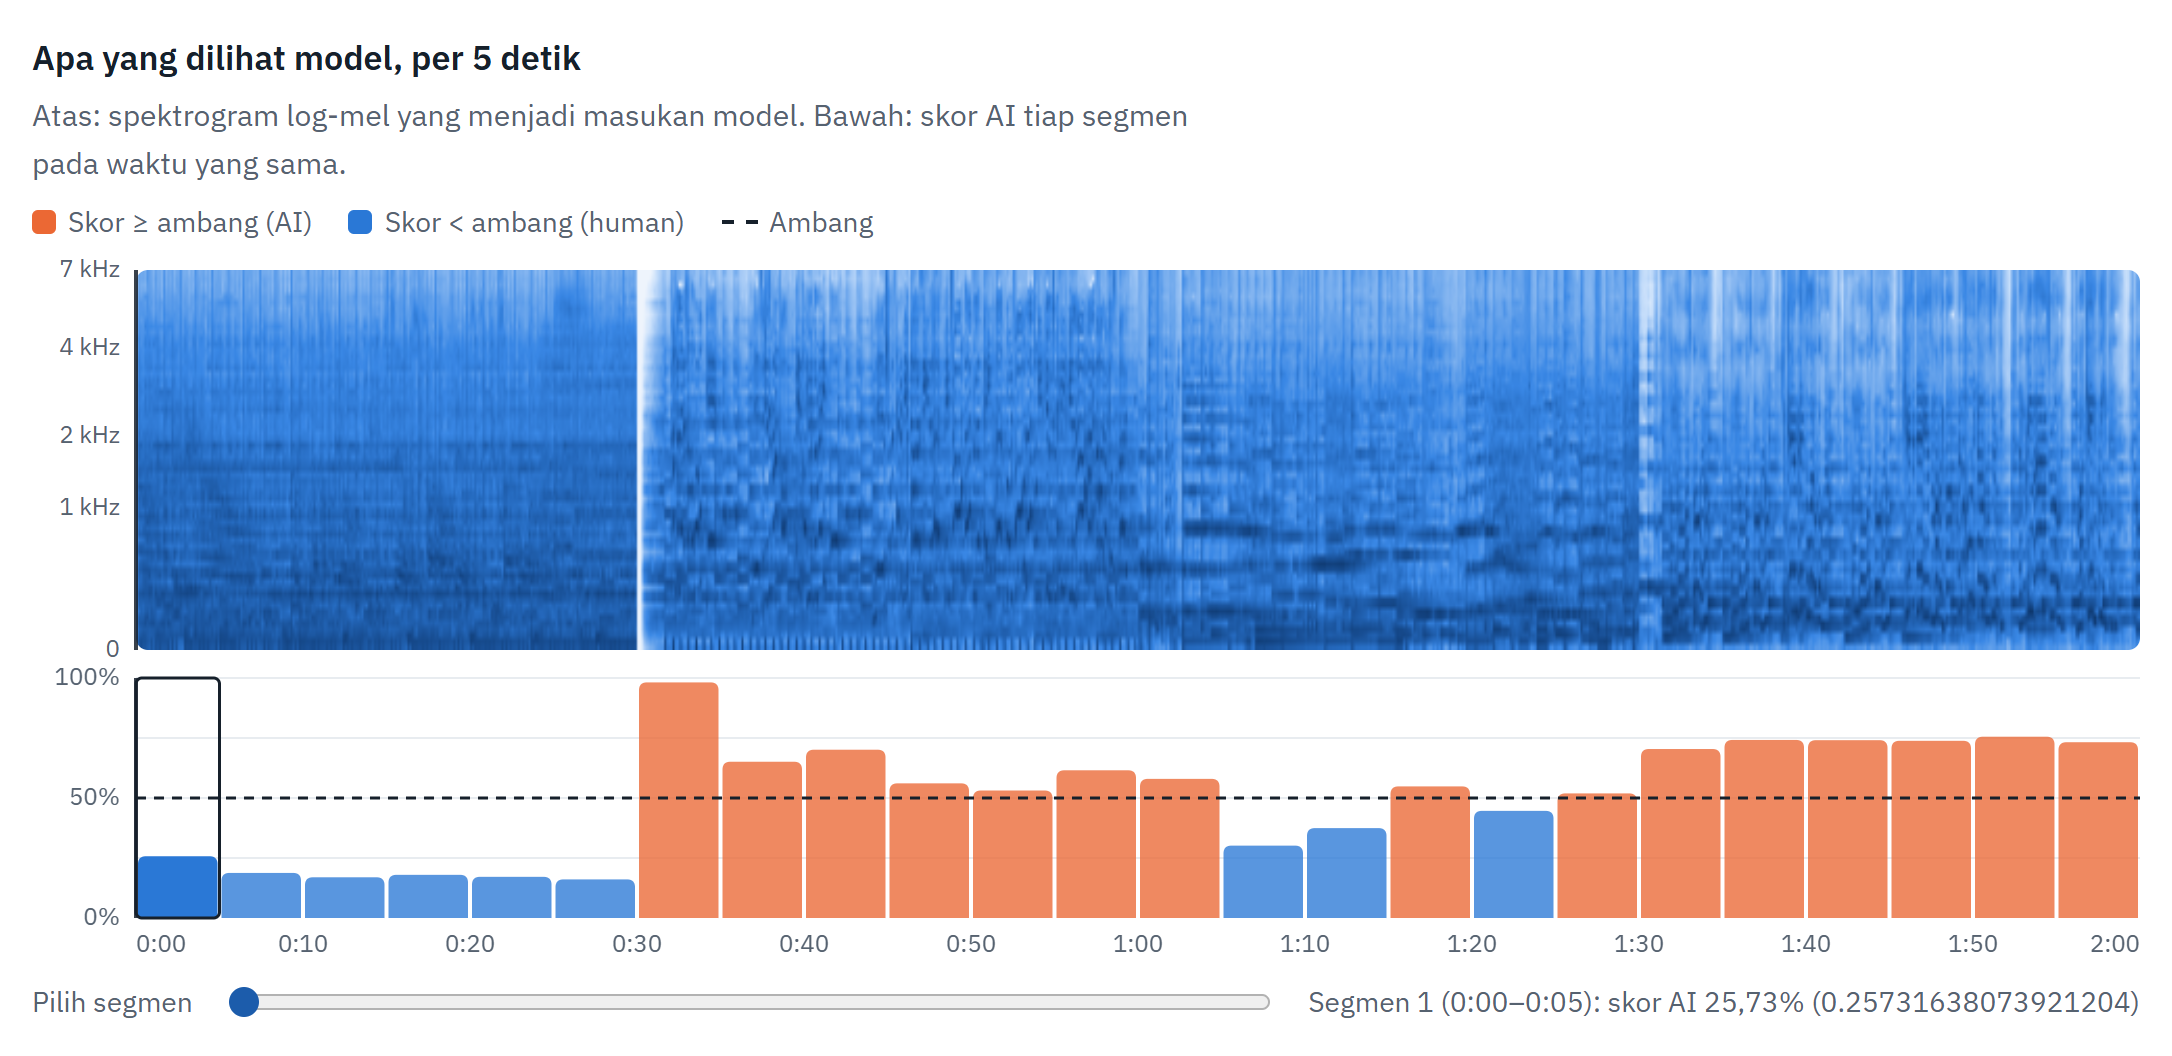
\includegraphics[width=0.95\textwidth]{04-spektrogram-skor.png}
\caption{Spektrogram log-Mel dan skor AI per segmen 5 detik pada sumbu waktu yang sama.}
\label{fig:spektrogram}
\end{figure}

\begin{figure}[htbp]
\centering
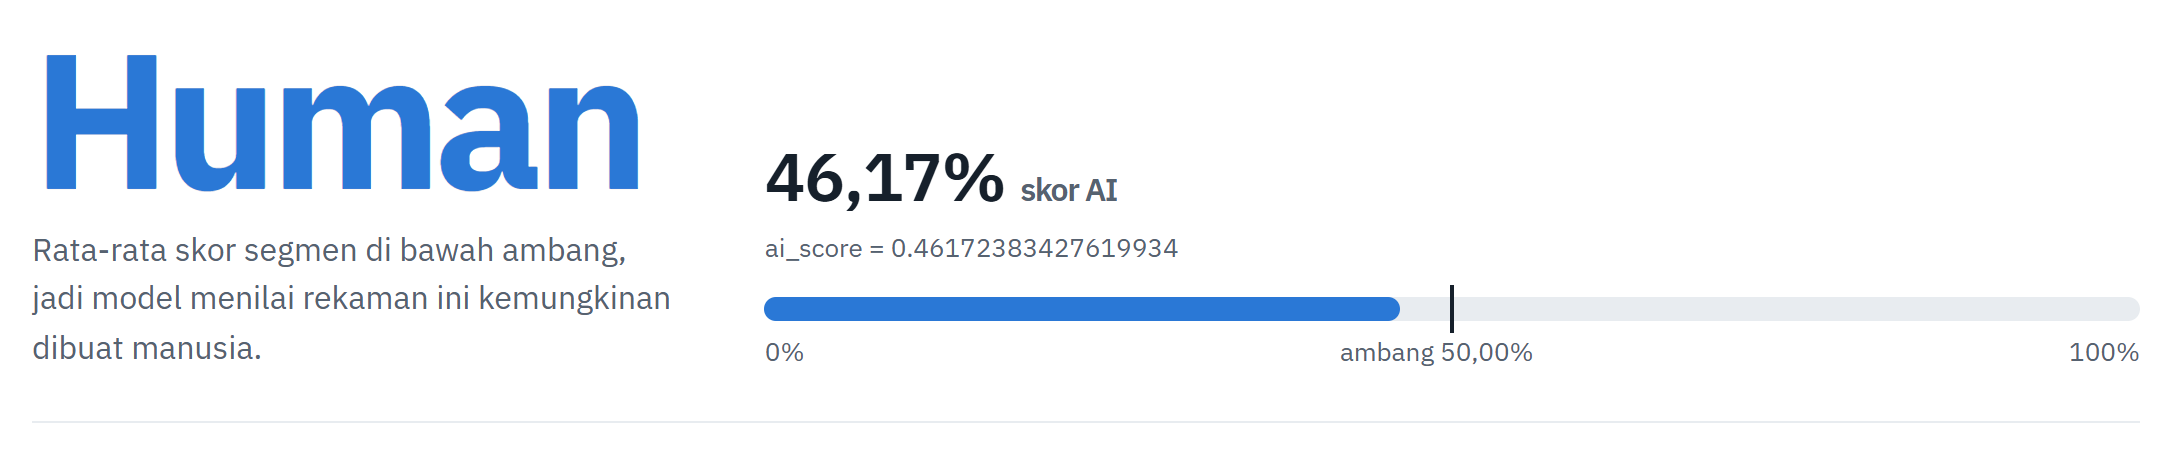
\includegraphics[width=0.95\textwidth]{08-contoh-human.png}
\caption{Contoh vonis Human untuk lagu FMA dengan skor 46,17\%.}
\label{fig:contoh-human}
\end{figure}

Studio juga dapat dibuka di layar ponsel; semua bagian tersusun dalam satu kolom (Gambar~\ref{fig:ponsel}). Laporan JSON berisi \kode{status}, \kode{filename}, \kode{result} (vonis, skor, ambang, cara agregasi, panjang dan jumlah segmen, serta skor per segmen), dan \kode{metadata} (arsitektur, nama run, dan waktu proses). Contoh lengkapnya ada pada Lampiran~C.

\begin{figure}[htbp]
\centering
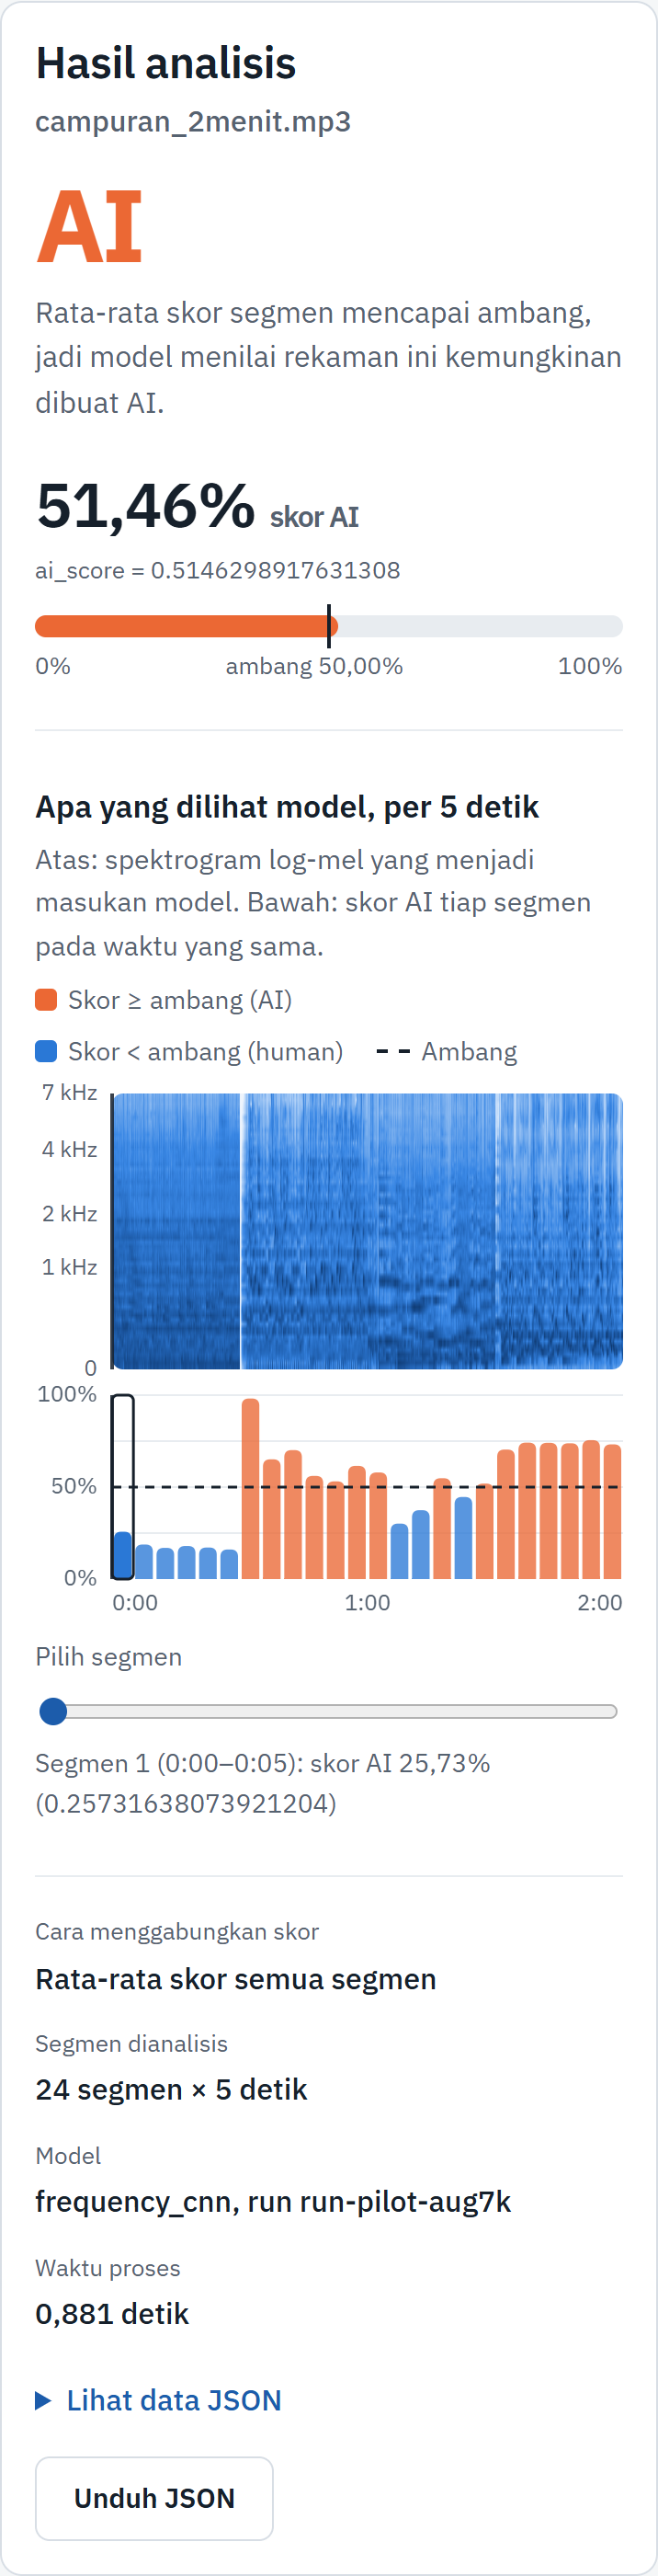
\includegraphics[height=0.62\textheight]{09-tampilan-hp.png}
\caption{Hasil analisis pada layar ponsel dengan lebar 390 piksel.}
\label{fig:ponsel}
\end{figure}

\section{Memberi Umpan Balik}
Setelah vonis muncul, pengguna dapat menandai apakah vonis itu benar. Kumpulan jawaban ini menjadi uji lapangan, yaitu ukuran seberapa sering model benar pada lagu sungguhan yang diperiksa pengguna.
\begin{enumerate}
\item Analisis lagu yang asal-usulnya diketahui.
\item Pada kartu \textbf{Apakah vonis ini benar?}, pilih \textbf{Benar}, \textbf{Salah}, atau \textbf{Tidak tahu}.
\item Untuk Benar atau Salah, pilih sumber label (wajib): dibuat sendiri, label resmi platform, dataset dengan asal-usul jelas, konfirmasi pembuat, atau lainnya.
\item Centang \textbf{Simpan salinan audio} hanya jika berhak menyimpannya dan ingin lagu itu dipakai untuk evaluasi atau pelatihan ulang.
\item Klik \textbf{Simpan umpan balik}. Untuk lagu dan model yang sama, jawaban terakhir yang dipakai.
\end{enumerate}

\begin{figure}[htbp]
\centering
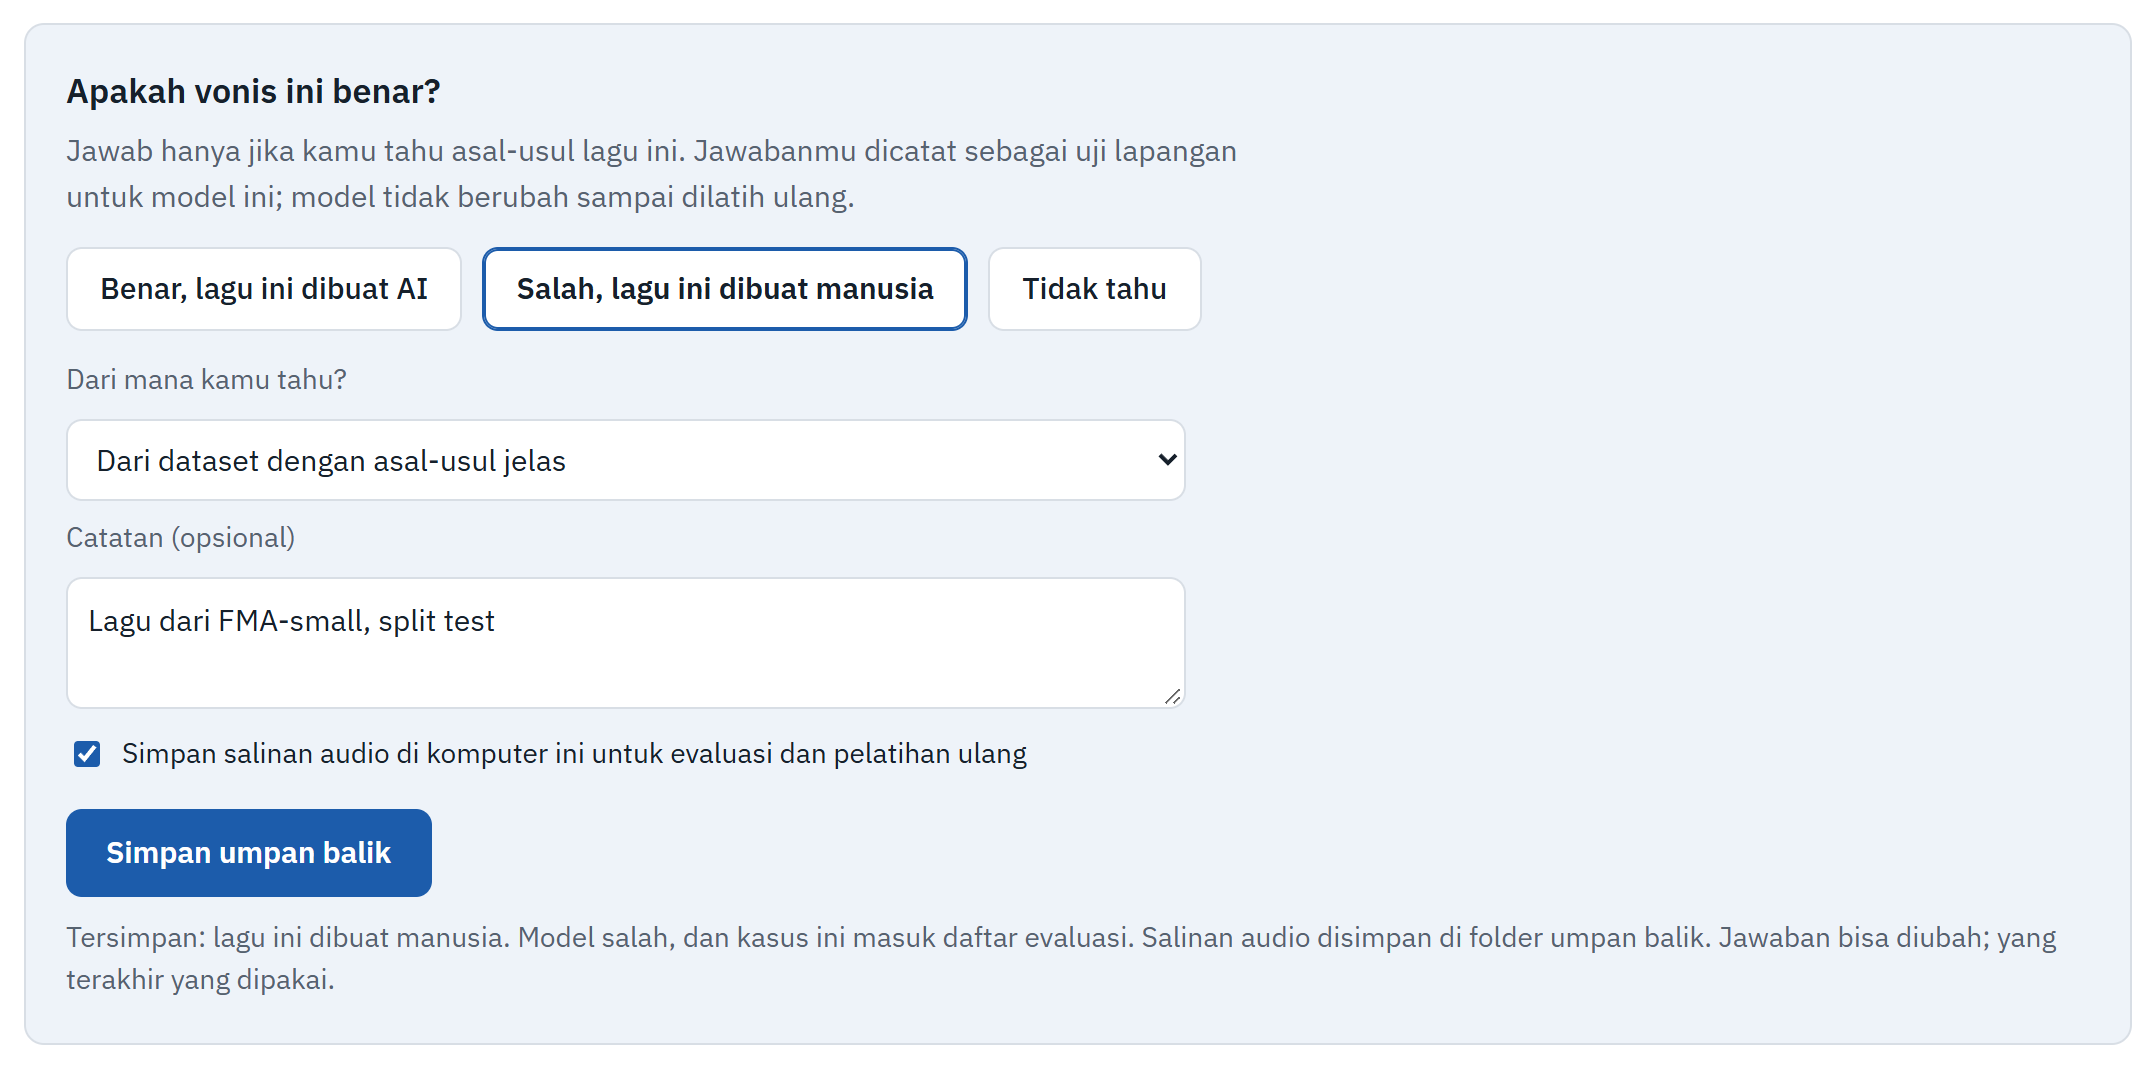
\includegraphics[width=0.9\textwidth]{11-umpan-balik-tersimpan.png}
\caption{Kartu umpan balik setelah disimpan.}
\label{fig:umpan-balik}
\end{figure}

Setiap jawaban disimpan sebagai satu baris di file \nolinkurl{data/feedback/feedback.jsonl}, berisi sidik jari file (SHA-256), nama file, nama run, vonis, skor, jawaban, label sebenarnya, sumber label, catatan, dan waktu. Panel \textbf{Uji lapangan} menampilkan akurasi beserta rentang 95\% Wilson, jumlah salah tuduh, jumlah lagu AI yang lolos, tabel benar dan salah, serta daftar kasus yang salah dinilai (Gambar~\ref{fig:uji-lapangan}).

\begin{figure}[htbp]
\centering
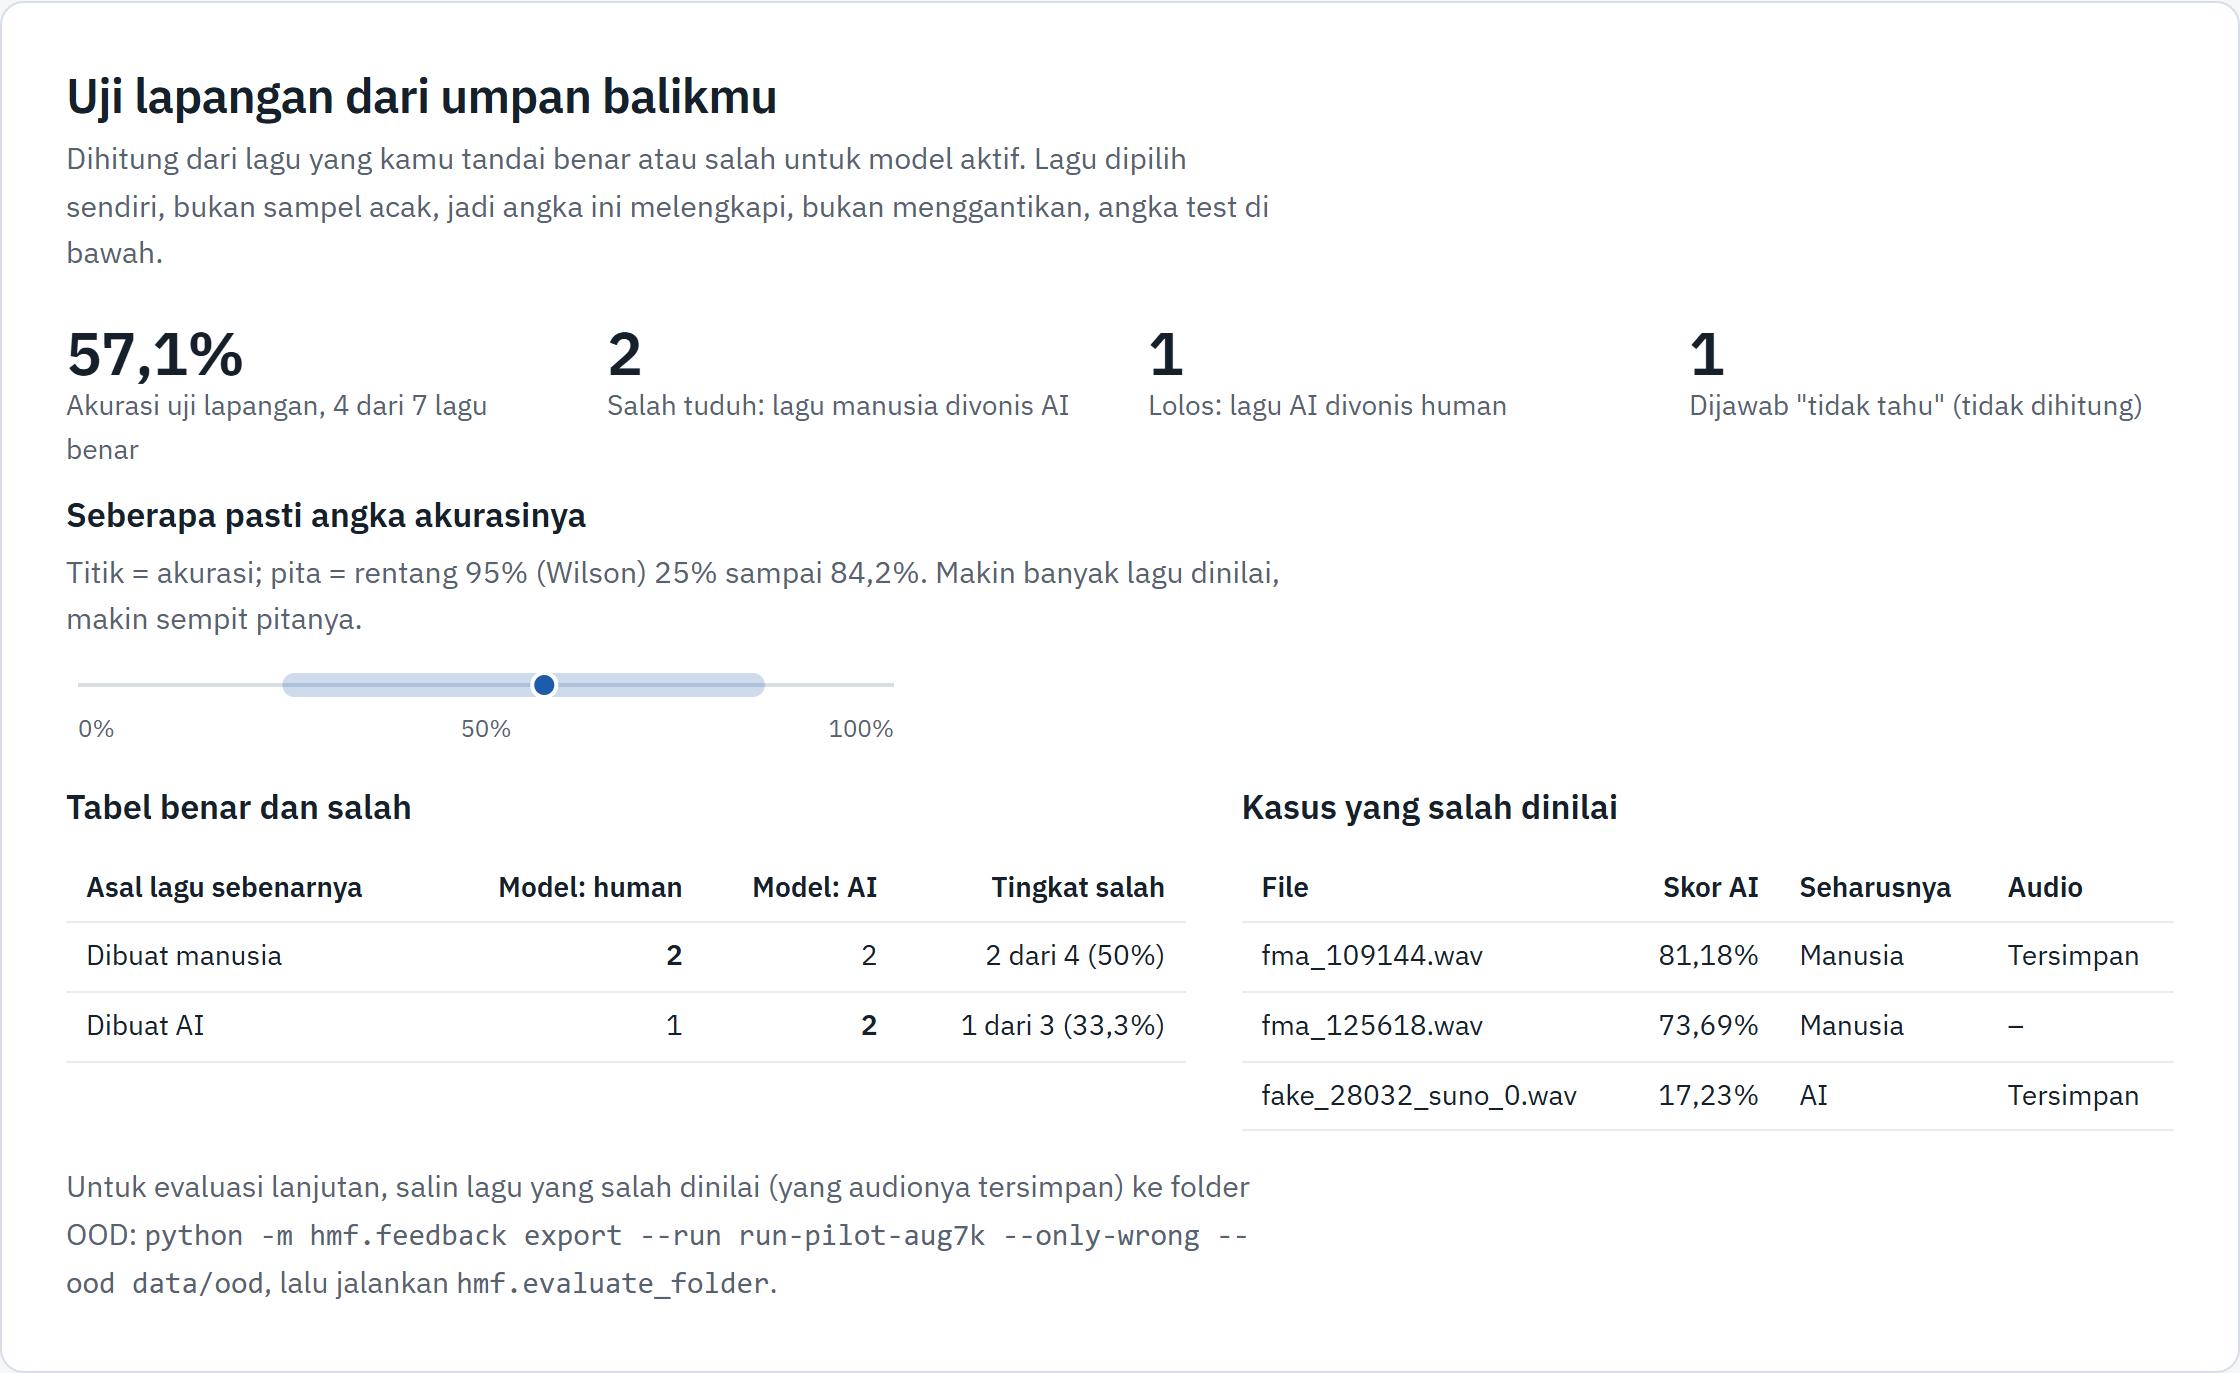
\includegraphics[width=0.95\textwidth]{12-uji-lapangan.png}
\caption{Panel uji lapangan: 4 dari 7 lagu benar dengan rentang 95\% 25--84\%.}
\label{fig:uji-lapangan}
\end{figure}

Lagu yang salah dinilai dapat dipakai untuk evaluasi lanjutan:
\begin{Perintah}
python -m hmf.feedback report --csv laporan.csv
python -m hmf.feedback export --run hmf-aug-v2 --only-wrong \
    --ood data/ood
python -m hmf.evaluate_folder --run runs/hmf-aug-v2 \
    --ai data/ood/ai --human data/ood/human
\end{Perintah}
Uji lapangan memiliki batasan: model tidak berubah sebelum dilatih ulang, lagu dipilih sendiri sehingga akurasinya tidak setara dengan angka test resmi, dan label berasal dari pengakuan pengguna. Lagu yang dipakai melatih ulang tidak boleh dipakai lagi untuk menguji model hasil pelatihan itu.

\section{Panel Tentang Model}
Panel di bagian bawah studio menunjukkan seberapa bisa dipercaya model yang aktif (Gambar~\ref{fig:panel-model}). Angkanya dibaca dari \kode{report.json} milik run tersebut dan diukur pada data test, bukan pada lagu yang diunggah. Panel memuat akurasi, \textit{balanced accuracy}, ROC AUC, jumlah lagu test, kurva loss train dan validasi per epoch, akurasi test per generator, serta konfigurasi audio. Akurasi per generator lebih berguna daripada akurasi total karena memperlihatkan generator yang sulit dideteksi.

\begin{figure}[htbp]
\centering
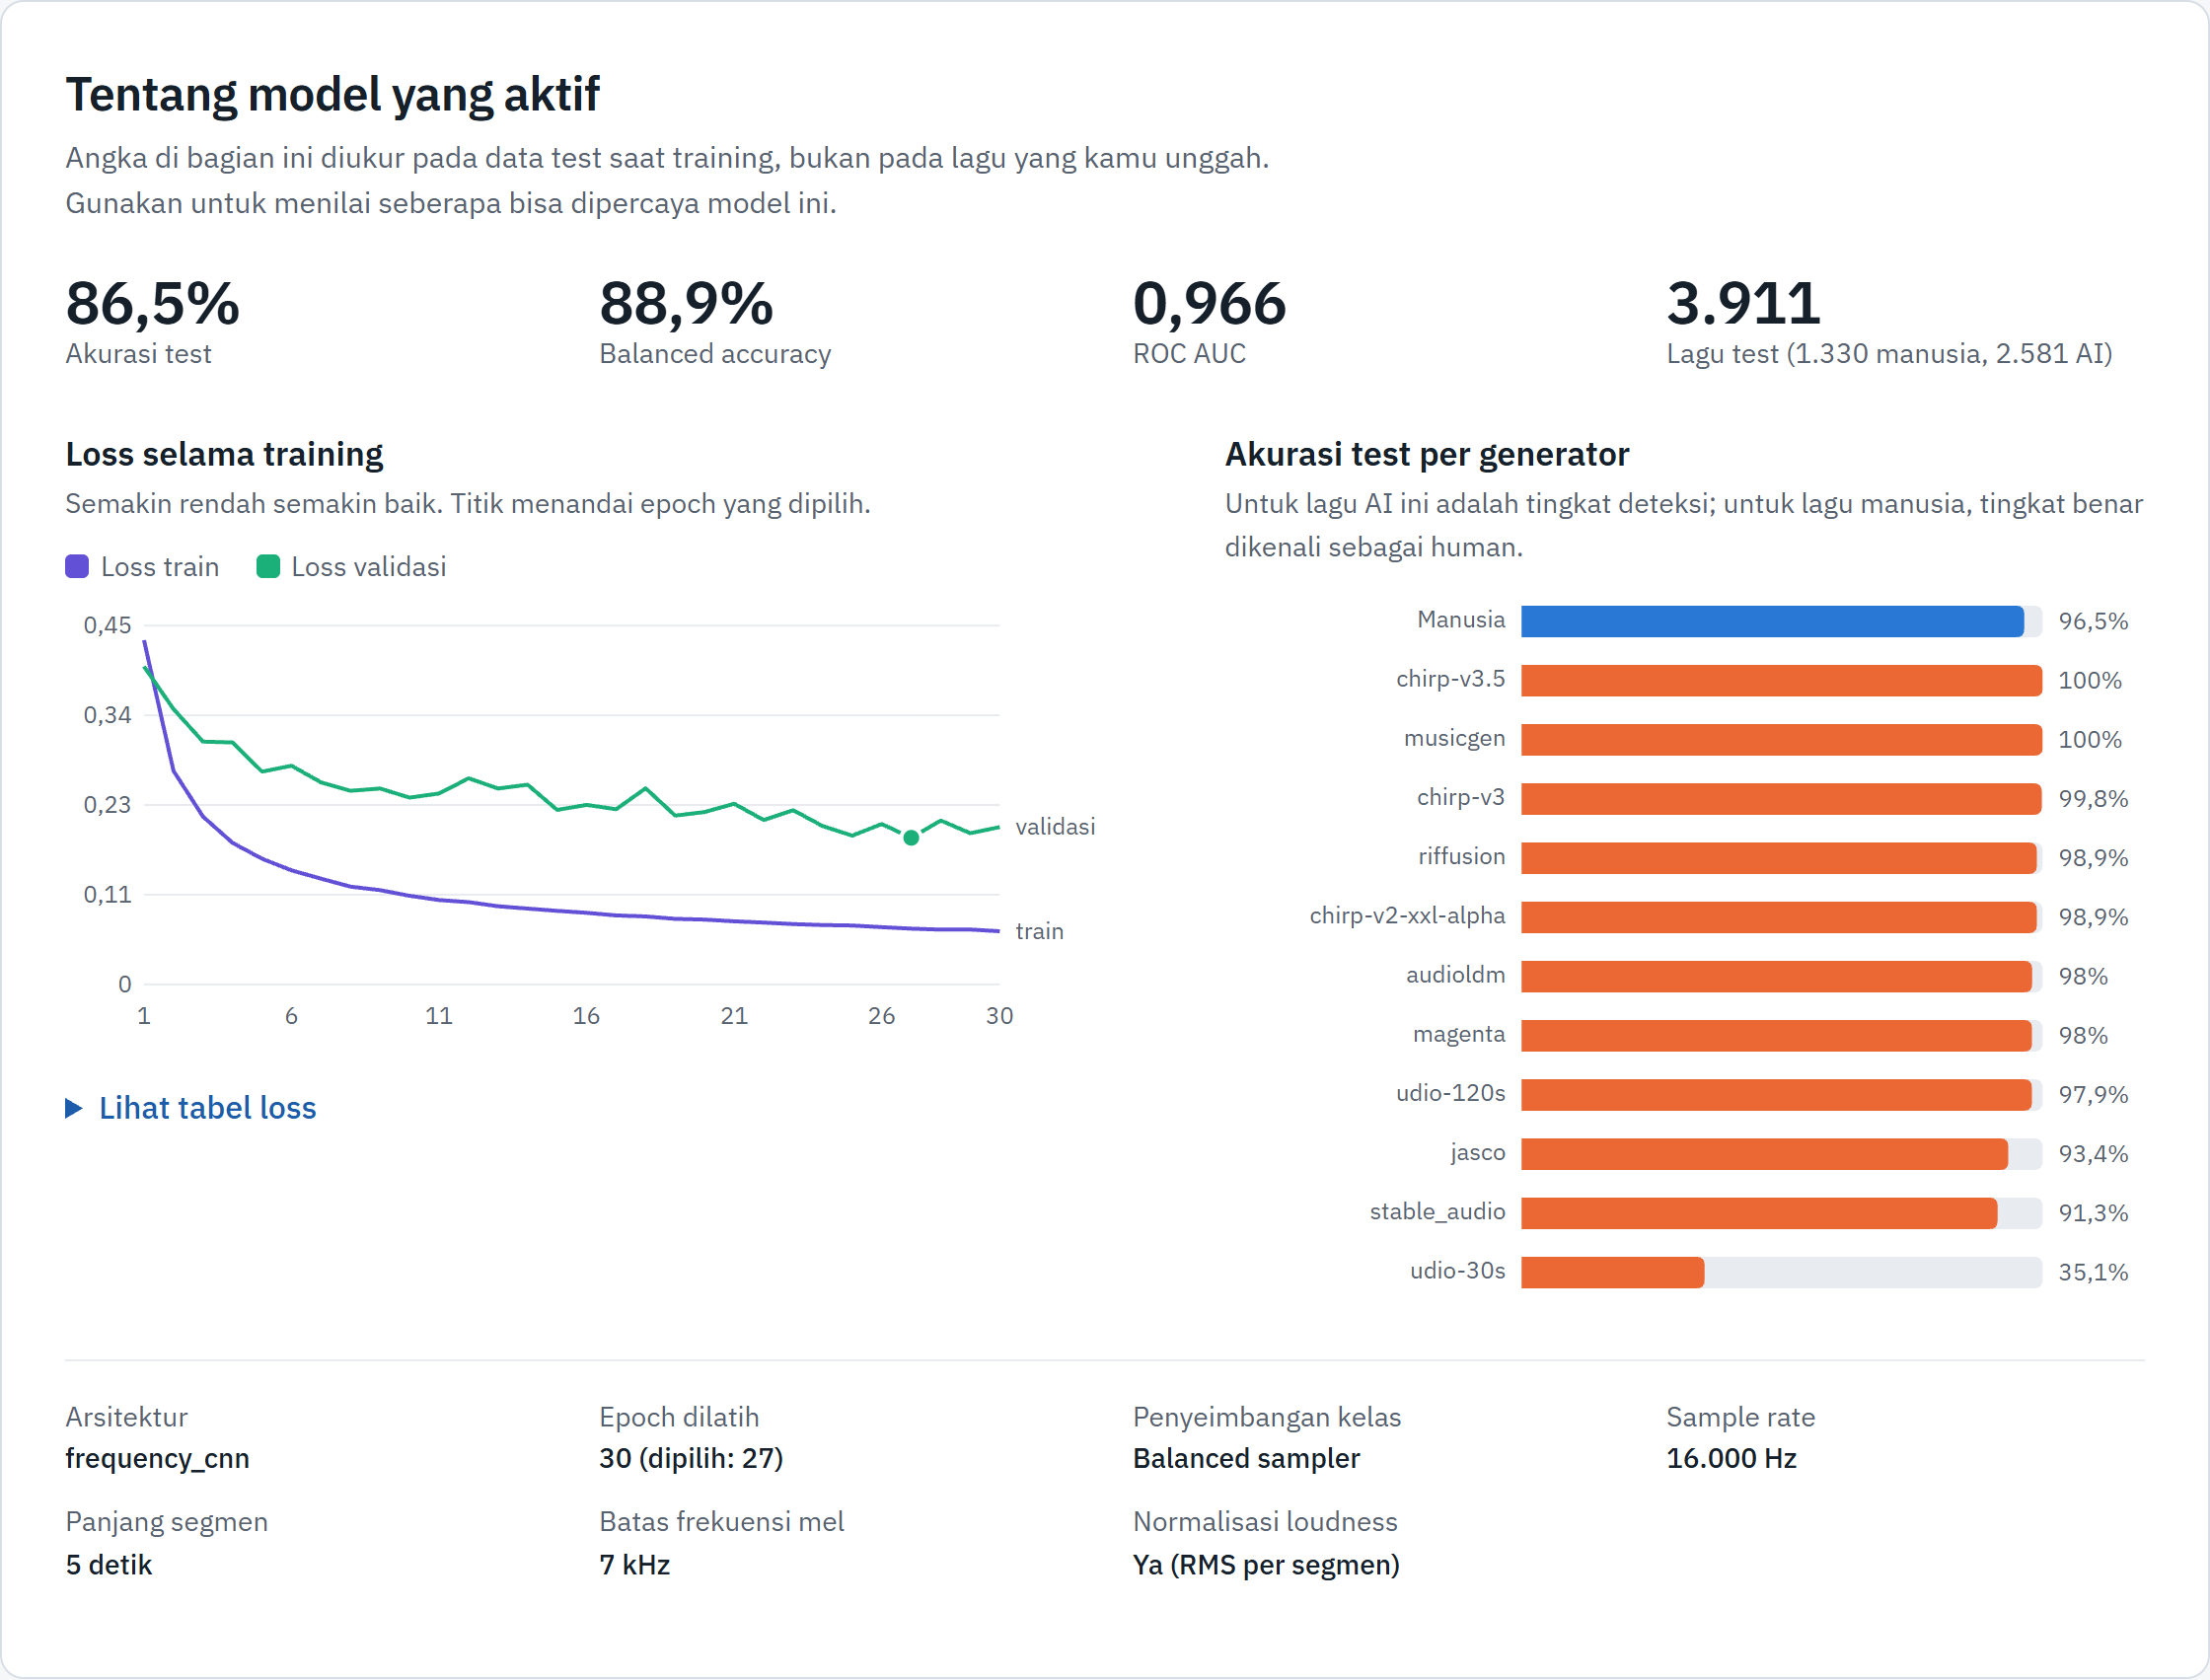
\includegraphics[width=0.95\textwidth]{06-tentang-model.png}
\caption{Panel Tentang model untuk model final \kode{hmf-aug-v2}.}
\label{fig:panel-model}
\end{figure}

\section{Melatih Ulang Model}
\begin{enumerate}
\item Unggah ke \kode{MyDrive/HMF/} di Google Drive: \kode{ai-music-detector-colab.zip} (kode dan manifest), \kode{fake\_songs.zip}, dan \kode{fma\_small.zip}.
\item Buka \kode{colab/train.ipynb} di Google Colab dan periksa sel konfigurasi (nama file, \kode{AUGMENT\_VARIANTS}, \kode{RUN\_NAME}).
\item \textbf{Sesi CPU:} jalankan semua sel dari atas. Notebook menyalin audio, mengunduh subset MUSEBENCH, membuat manifest, lalu menyiapkan fitur per 1.000 lagu. Setiap 100 lagu yang selesai disimpan ke Google Drive.
\item Jika sesi terputus, jalankan notebook lagi dari atas. Lagu yang sudah selesai tidak diproses ulang. Ulangi sampai muncul \kode{PREPARE SELESAI}.
\item \textbf{Sesi GPU:} ganti runtime ke GPU dan jalankan lagi dari atas. Pelatihan, uji \textit{robustness}, dan evaluasi OOD berjalan; pelatihan yang terhenti dilanjutkan otomatis dari epoch terakhir.
\item Salin folder \kode{MyDrive/HMF/runs/<RUN\_NAME>} ke folder \kode{runs/} di laptop, lalu buka dengan studio.
\end{enumerate}
Perintah inti tanpa notebook:
\begin{Perintah}
python -m hmf.manifest musebench --root <folder> \
    --reference-manifest data/manifest-28000.csv
python -m hmf.prepare --manifest <csv> --output <cache> \
    --augment-variants 3 --max-segments 6 --loudness-norm \
    --fmax 7000 --float16 --drop-duplicates \
    --resume --max-new-tracks 1000
python -m hmf.train --cache <cache> --output runs/<nama> \
    --epochs 30 --batch-size 64 --model frequency \
    --monitor loss --balance sampler \
    --balance-by generator --resume
\end{Perintah}
Cache fitur float16 berukuran $\pm$42 KB per segmen; dengan 3 varian dan 6 segmen per lagu, totalnya $\pm$20--25 GB untuk $\pm$36.000 lagu.

\section{Pemecahan Masalah}

{\singlespacing\small
\begin{longtable}{L{4.1cm} L{3.8cm} L{4.4cm}}
\caption{Pemecahan masalah umum.}\label{tab:masalah}\\
\toprule
Gejala & Penyebab & Solusi\\
\midrule
\endfirsthead
\toprule
Gejala & Penyebab & Solusi\\
\midrule
\endhead
\bottomrule
\endfoot
Port 8765 sudah dipakai & Studio lain masih berjalan & Hentikan studio lama dengan Ctrl+C atau pakai \kode{--port 8800}\\
Tidak ada run lengkap & Folder \kode{runs/} kosong atau run belum selesai & Salin folder run ke \kode{runs/} atau pilih dengan \kode{--run}\\
Audio gagal dibaca & Format tidak didukung atau file rusak & Konversi ke MP3 atau WAV, lalu coba lagi\\
File lebih dari 32 MB & Batas unggah studio & Potong rekaman atau kompres ke MP3\\
Pemutar audio tidak muncul & Browser tidak dapat memutar format itu & Analisis tetap dapat dijalankan\\
Skor berbeda dari sebelumnya & Model aktif berbeda & Periksa nama run di pojok kanan atas\\
Tidak dapat terhubung ke GPU di Colab & Kuota GPU gratis habis & Siapkan fitur di runtime CPU; lanjutkan pelatihan saat kuota kembali\\
Disk penuh saat menulis cache & Disk Colab tidak cukup & Kurangi \kode{AUGMENT\_VARIANTS} atau jumlah lagu MUSEBENCH sebelum sesi pertama\\
Duplicate audio bytes & File yang sama muncul dua kali & Tambahkan \kode{--drop-duplicates}\\
Pengaturan berbeda dari plan & Pengaturan diubah di tengah cicilan & Kembalikan pengaturan atau pakai \kode{RUN\_NAME} baru\\
\end{longtable}}
